% ==================================================
\section{Losses}
\label{methods:losses}
To train the generator function~\ref{equation:predictor-loss-minimization}, we tried several loss functions $\SL$ that are commonly used for image restoration~\citep{zhao2016loss}. It is not clear which one is optimal: since the resulting image will be evaluated by a human observer, as we need to use perceptually motivated losses. Sometimes, multiple loss functions are combined to produce a more sophisticated one~\citep{zhao2016loss}. In our experiments, the loss functions are used both for training and evaluation as \textit{accuracy} metrics.


% **************************************************
\subsection{L1}
\label{methods:losses:L1}

$L_1$ loss, also known as the mean absolute error (MAE), is a measure of the difference between two continuous variables. This loss function can be used in regression analysis to evaluate the accuracy of a predictive model.

The $L_1$ loss of the predicted value $\hat{y}$ and the true value $y$ is defined as:

\begin{equation}
L_1(\hat{y},y) = |\hat{y} - y|\:.
\end{equation}

The $L_1$ loss is a pixel-wise loss that computes the absolute difference between predicted and true values, which is then averaged across pixels.  It has the property of being robust to outliers, as the loss is not affected by large differences between the predicted and true values. The interpretability of this loss function is especially evident when compared with other loss functions that we use.


% **************************************************
\subsection{MSE}
\label{methods:losses:MSE}
Mean squared error (MSE) is a loss function used in regression analysis to evaluate the accuracy of a model. It measures the average squared difference between the predicted and true values.

The MSE between the predicted value $\hat{y}$ and the true value $y$ is defined as:

\begin{equation}
MSE(\hat{y},y) = (\hat{y} - y)^2\:.
\end{equation}

The squared difference between the predicted and true values penalizes large errors more than small errors. It is another possible choice for regression problems where the goal is to minimize the average squared difference between the predicted and true real values. This loss function is computed pixel-wise and then averaged across all the pixels.


% **************************************************
\subsection{SSIM}
\label{methods:losses:SSIM}
The structural similarity (SSIM) index is a popular loss function used in image processing to measure the similarity between two images. It compares the structural information of the images, including luminance, contrast, and structure. The first definition was presented in~\citep{wang2004image}.

The SSIM index between two images $x$ and $y$ is defined as:

\begin{equation}
SSIM(x,y) = \frac{(2\mu_x\mu_y + c_1)(2\sigma_{xy} + c_2)}{(\mu_x^2 + \mu_y^2 + c_1)(\sigma_x^2 + \sigma_y^2 + c_2)}\:,
\end{equation}

where $\mu_x$ and $\mu_y$ are the mean values of images $x$ and $y$, $\sigma_x$ and $\sigma_y$ are the standard deviations of images $x$ and $y$, and $\sigma_{xy}$ is the cross-covariance between $x$ and $y$. The constants $c_1$ and $c_2$ are small constants added to stabilize the division and are typically set to $c_1=(k_1L)^2$ and $c_2=(k_2L)^2$, where $L$ is the dynamic range of the pixel values and $k_1$ and $k_2$ are constants.

The SSIM index ranges between 0 and 1, where a value of 1 indicates perfect similarity between the two images.

The SSIM loss between two images $x$ and $y$ is defined as:

\begin{equation}
L_{SSIM}(x,y) = 1 - SSIM(x,y)\:.
\end{equation}

This measures the dissimilarity between the two images, with a value of 0 indicating perfect similarity.

The advantage over $L_1$~\ref{methods:losses:L1} or MSE~\ref{methods:losses:MSE} is that it takes into account the perceptual quality of the image, rather than just pixel-wise differences.
One of the disadvantages of this loss is the necessity to determine a window size/resolution scale, at which the loss is computed. This is solved by the MSSSIM loss~\ref{methods:losses:MSSSIM}.


% **************************************************
\subsection{MSSSIM}
\label{methods:losses:MSSSIM}
The multiscale structural similarity (MSSSIM) index is an extension of the SSIM index that takes into account the multi-scale nature of image perception. It was first defined in~\citep{wang2003multiscale}. It compares the structural information of images at different scales, providing a more accurate measurement of image similarity.

The MSSSIM index between two images $x$ and $y$ is defined as:

\begin{equation}
MSSSIM(x,y) = \frac{1}{n}\sum_{i=1}^{n} w_i \cdot SSIM(x_i, y_i)\:,
\end{equation}

where $n$ is the number of scales, $x_i$ and $y_i$ are the images at the $i$-th scale, and $w_i$ is a weight parameter that depends on the scale. The weights are typically chosen to be a Gaussian function of the scale, with the largest weight assigned to the lowest scale.

The MSSSIM loss between two images $x$ and $y$ is defined as:

\begin{equation}
L_{MSSSIM}(x,y) = 1 - MSSSIM(x,y)\:.
\end{equation}

This measures the dissimilarity between the two images, with a value of 0 indicating perfect similarity.

MSSSIM loss is commonly used as a loss function in deep learning algorithms for image processing tasks such as image denoising~\citep{bera2019lightweight}, super-resolution~\citep{min2023d}, and image restoration~\citep{zhao2016loss}. It is preferred over other loss functions such as mean squared error and SSIM as it provides a more accurate measurement of image similarity by taking into account the multi-scale nature of image perception.


% **************************************************
\subsection{MIX: a loss combining $L_1$ and MSSSIM}
\label{methods:losses:MIX}
Similarly as in~\citep{zhao2016loss}, we implemented also a loss combined from $L_1$~\ref{methods:losses:L1} and MSSSIM loss~\ref{methods:losses:MSSSIM}. In the paper, a Gaussian function is used to give more weight to the central part of the image for the $L_1$ loss. As we do not use this, in our case the final loss is defined as:


\begin{equation}
L_{MIX}(x,y) = \alpha \cdot L_{MSSSIM}(x,y) + (1 - \alpha) \cdot L_1(x,y)\:,
\end{equation}
where the value of $\alpha$ is set as described in the paper~\citep{zhao2016loss} to $0.84$.


% **************************************************
\subsection{Discriminator}
\label{methods:losses:adversarial}
We tried also a more sophisticated loss function common in training Generative Adversarial Networks (GANs)~\citep{goodfellow2014generative}, which was implemented using a CNN network. The discriminator network is responsible for determining whether the input image is real or fake. The use of discriminator loss has been shown to improve the quality of generated images~\citep{radford2015unsupervised, ledig2017photorealistic, wang2018highresolution}.

The model has multiple convolutional layers, with an increasing number of filters. The input image size is expected to be 110x110 pixels and the final output is a single value between 0 and 1, which represents the probability that the input image is real. The leaky ReLU activation function is used after each convolutional layer, except for the final layer where the sigmoid activation function is used to produce the probability score. The architecture is presented in picture~\ref{img:methods:losses:adversarial}.

The total number of trainable parameters in the model is 6,300,865.

If we define an objective function for the discriminator $\ell \colon \SX \rightarrow [0,1]$ as
\begin{equation}
  \label{equ:generator_quality_2}
  \begin{array}{rl}
  F_\ell(\#\omega_g,\#\omega_\ell) = \displaystyle\frac{1}{m}\sum_{j=1}^m \big(\log (1 - \ell(g( x^j; \#\omega_g); \#\omega_\ell )) + \log \ell( s^j; \#\omega_\ell) \big) \:,
  \end{array}
\end{equation}

where $s \in \SX$ is the desired stimuli image, $g$ is the generator function defined in~\ref{methods:models:problem-definition}, $\#\omega_g$ are its trained parameters and $\#\omega_\ell$ are the parameters of the discriminator function.

The output value of the discriminator $\ell(x; \#\omega_\ell)$ corresponds to the probability, that the image $x \in \SX$ is a real image, the value $1 - \ell(x; \#\omega_l)$ corresponds to the probability that the image $x \in \SX$ is a synthetic image generated by the generator function $g$. The convolutional network implementing the discriminator function contains a sigmoid function at the end to produce the probability.

We find the parameters $\#\omega_\ell$ and $\#\omega_g$ by solving a minimax problem:
\begin{equation}
   \label{equ:minimax}
    (\#\omega^*_g, \#\omega_\ell^*) \leftarrow \min_{\#\omega_g}\max_{\#\omega_\ell} 
    F_\ell(\#\omega_g, \#\omega_\ell) \:.
\end{equation}
To solve~\ref{equ:minimax}, we minimize~\ref{equ:generator_quality_2} with respect to $\#\omega_g$ when $\#\omega_\ell$ is fixed to find the best parameters for the generator function $g$ and alternate this step with maximization with respect to $\#\omega_\ell$ when we use fixed $\#\omega_g$ parameters to find the best parameters for the discriminator function $\ell$.

\begin{figure}[H]\centering
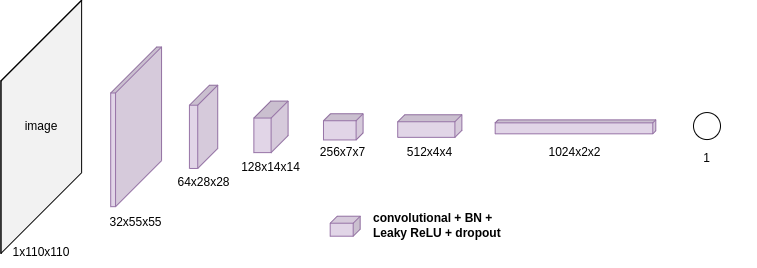
\includegraphics[width=140mm]{img/discriminator.drawio.png}
\caption{CNN architecture of the discriminator.}
\label{img:methods:losses:adversarial}
\end{figure}

To further improve the quality of the generated images, we use discriminator loss together with MSSSIM loss during training. The discriminator loss encourages the generated images to be indistinguishable from real images, while the MSSSIM forces the network to learn features that are based on the cortical activity. We selected a weights of $0.8$ for the discriminator loss and $0.2$ for the MSSSIM loss to balance the two objectives.
